\chapter{Execute Stage}

\section{ALU: Arithmetic Logic Unit}
\subsection{Adder}
\subsection{Multiplier}
\subsection{Logic Operands}
\subsection{Shifting}
The implemented shifter allows to perform shift right, logical/arithmetical shift left and left/right rotate using the full operand \texttt{A} on 32 bits and 6 bits from the second one \texttt{B} and three \textit{control signals}.
Differently from the T2 version, it uses and addition signal in order to be able to manage also the rotate instruction. Our implementation takes three inputs:
\begin{itemize}
	\itemsep0sp
	\item \texttt{A}: the operand to be shifted/rotated;
	\item \texttt{B}: only the 5 LSB [4,3,2,1,0] are used to select first the mask to be used and then the starting point from that mask;
	\item \texttt{SEL}: it encodes the operation type; the second bit is used to select among arithmetic and logic, the third bit is used to select the direction of the shift/rotate (left/right) and the first one is used only if the operation is a rotate. This is the encoding:
	\begin{center}
		\begin{tabular}{c|l}
			\texttt{SEL} & \textbf{Operation}\\
			\hline
			000 & Shift logic right \\
			001 & Shift logic left \\
			010 & Shift arith right \\
			011 & Shift arith left \\
			100 & Rotate right \\
			101 & Shift right \\
		\end{tabular}
	\end{center}
\end{itemize}

 The unit perform the requested operation in three stages:
\begin{enumerate}
	\item The first consist in preparing 4 possible ``masks", each already shifted of {0, 8, 16, 32} left
	or right depending on the configuration. This allows to shift for all 32 bits. Basically it copies
	the input \texttt{A} into the 4 masks that will be used by the next stage. Being in 32 bits, the generated masks are in $32+8=40$ bits. The only different between this implementation and the T2 one, is that, in case of rotate, the additional 8 bits of the masks are filled with the corresponding 8 bits that are going ``out" during the rotation.
	
	\item The second level perform a coarse grain shift, that is basically consist on selecting one mask
	among the 4 possible masks generated in the previous stage. This selection is done by using the bits {4, 3} of \texttt{B}.
	\item The third level, using the bits {2, 1, 0} of \texttt{B} and the selected mask, preform a fine grain refinement. The 3 bits allows to select the starting index from the mask, in fact it allows to select among 8 positions.
\end{enumerate}

\begin{figure}[ht]
	\centering
	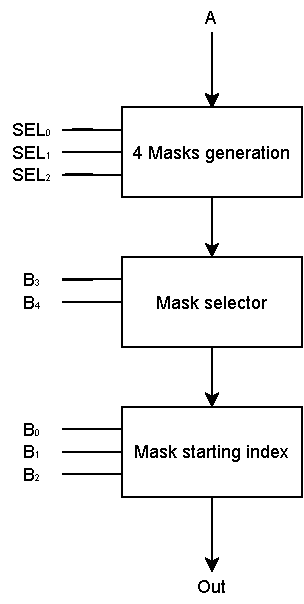
\includegraphics[width=0.2\textwidth]{chapters/5_ExecuteStage/images/Shifter.pdf}
	\caption{Blocks of the Shifter/Rotate Unit}
	\label{shifter}
\end{figure}


\begin{mybox}
	\textbf{Examples}
	\newline
	For example, if we need to perform a left left of 9 bits \texttt{A}, where \texttt{A=18}, the corresponding \texttt{B} value will be 1001; this means that the second masks will be taken and the output result will from the bit at position $40-1=39$ to the one at $39-32=7$ included.
	\begin{center}
		MASK 2: 0$\underbrace{\textbf{0000000 00000000 00000000 00010010 0}}_{\text{shifted \texttt{A}}}$0000000
	\end{center}
	
	On the other hand, if we need to perform a right shift the masks are generated in the opposite way, so the zeros are put in the MSB of the mask, shifted by 0, 8 ... positions. In this case we need also to distinguish between the an arithmetic and a logic shift; in the first case, instead of filling the ``empty" bits with zero, the operand sign is used. For example, if we want to shift \texttt{A=-18} of \texttt{B=3} bits, the first mask is used: 
	\begin{center}
		MASK 1: 11111$\underbrace{\textbf{111 11111111 11111111 11111111 11101}}_{\text{shifted \texttt{A}}}$110
	\end{center}
	
	In the last case, let's suppose to rotate right \texttt{A=1255} (=10011100111) by 5 position:
	\begin{center}
		MASK 1: 11$\underbrace{\textbf{100111 00000000 00000000 0000100 111}}_{\text{rotated \texttt{A}}}$00111
	\end{center}
	As you can see, in case of MASK 1 for the right rotation, the 8 LSB of \texttt{A} are copied into the 8 MSB of the mask.
\end{mybox}
	

\section{Set-Like Operations unit}
- setcmp